\documentclass[aspectratio=43]{beamer}

\definecolor{theme}{RGB}{28,90,127}
\definecolor{offblack}{HTML}{262626}
\definecolor{emph}{HTML}{00A7DA}
\setbeamercolor{normal text}{fg=offblack}

% change text to offblack
\definecolor{almostblack}{HTML}{262626}
\definecolor{gunmetal}{HTML}{5C5858}
\definecolor{pyred}{HTML}{F24532}
\definecolor{pyblue}{HTML}{2E7EBC}
\definecolor{pyorange}{HTML}{FEA862}
\definecolor{theme}{RGB}{90,122,163}

\usecolortheme[named=theme]{structure}
\usecolortheme{rose}
\usecolortheme{dolphin}

\makeatletter
\setbeamertemplate{frametitle}{
  \ifbeamercolorempty[bg]{frametitle}{}{\nointerlineskip}%
  \@tempdima=\textwidth%
  \advance\@tempdima by\beamer@leftmargin%
  \advance\@tempdima by\beamer@rightmargin%
  \begin{beamercolorbox}[sep=0.3cm, left, wd=\the\@tempdima]{frametitle}
    \usebeamerfont{frametitle}
    \vbox{}\vskip-2ex%
    \if@tempswa\else\csname beamer@fteleft\endcsname\fi%
    \strut\insertframetitle\strut\par%
    {%
      \ifx\insertframesubtitle\@empty%
      \else%
      {\usebeamerfont{framesubtitle}\usebeamercolor[fg]{
        framesubtitle}\insertframesubtitle\strut\par}%
      \fi
    }%
    \vskip.45ex%
    \hrule %height .6pt%
    \vskip-1.45ex%
    \if@tempswa\else\vskip-.3cm\fi%
  \end{beamercolorbox}%
}
\makeatother

% clean up footer
\beamertemplatenavigationsymbolsempty
\setbeamertemplate{footline}[text line]{
  \parbox{\linewidth}{\vspace*{-10pt}
  \raggedleft \color{offblack} 
  \bf J.\ Scott Moreland (Duke U.)
  \quad \insertframenumber\,/\,\inserttotalframenumber}
}

%inner theme
\useinnertheme{rectangles}
\setbeamertemplate{itemize item}{
  \raise.30ex\hbox{\vrule width .80ex height .80ex}}
\setbeamertemplate{itemize subitem}{
  \raise.35ex\hbox{\vrule width .70ex height .70ex}}

% for backup slides
\usepackage{appendixnumberbeamer}
\renewcommand\appendixname{Backup}

\usepackage{graphicx}
\usepackage[absolute, overlay]{textpos}
\graphicspath{{fig/}}

\usepackage{amsmath}
\usepackage{amssymb}
\usepackage{tikz}
\usepackage{tikzscale}
\usetikzlibrary{calc}
\usetikzlibrary{fit}
\usetikzlibrary{positioning}

\usepackage[T1]{fontenc}
\usepackage[default]{lato}
\usepackage{tcolorbox}

\theoremstyle{definition}
\newtheorem{assertion}{Simplifying postulates}

\newcommand{\trento}{T\raisebox{-0.3ex}{R}ENTo}
\newcommand{\conference}{Quark Matter, Chicago, USA}

\title{Flow in small and large QGP droplets:\\
role of nucleon substructure}
\author[J.\ S.\ Moreland]{
  J.\ S.\ Moreland, J.\ E.\ Bernhard, W.\ Ke, S.\ A.\ Bass}
\institute[Duke]{Duke University}
\date{8 February 2017} 

\begin{document}

\section{Title}

\begin{frame}[plain, noframenumbering]
  \centering
  {\color{theme}\Large\inserttitle} \\[2ex]
  \insertauthor \\
  (\insertinstitute) \\[2ex]
  \scriptsize
  \conference \\
  \insertdate \\
  
\includegraphics{title_page} \\[2ex]

  \begin{textblock*}{\paperwidth}(0 cm, 8.3 cm)
    \scriptsize Funding provided by DOE NNSA Stewardship Science Graduate Fellowship \\
    Computing resources provided by the Open Science Grid,\\
    supported by the NSF and DOE Office of Science
  \end{textblock*}
\end{frame}


\begin{frame}[plain]{Success of saturation models + hydro}
  \centering
  \medskip
  \scriptsize Hydro models with saturation IC, e.g.\ \trento, IP-Glasma and EKRT,\\
  provide excellent description of bulk observables in A+A collisions \\[1ex]
  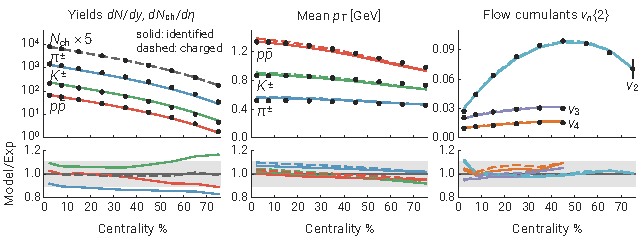
\includegraphics[width=.8\textwidth]{mode_observables} \\[1ex]
  \begin{textblock*}{0.3\textwidth}(9.5 cm, 2.0 cm)
    \rotatebox{-90}{\tiny PRC 94, 024907 [1605.03954]}
  \end{textblock*}
  \begin{columns}
    \begin{column}{.075\textwidth}
    \end{column}
    \begin{column}{.45\textwidth}
      \centering
      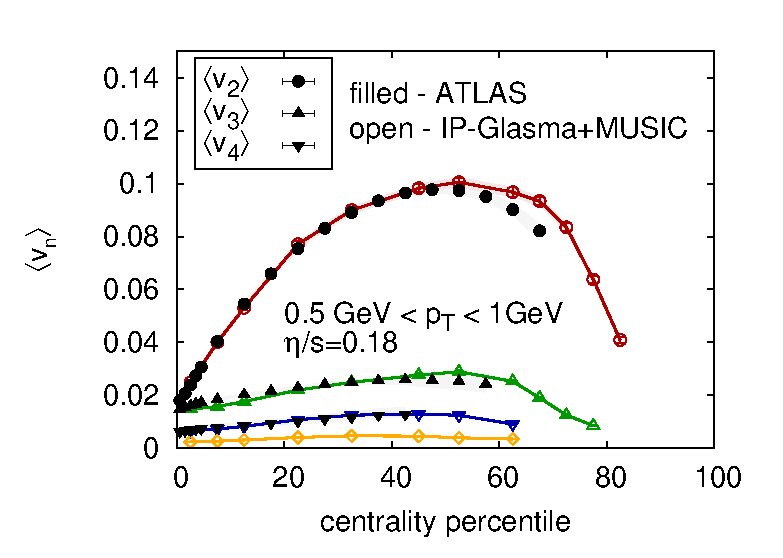
\includegraphics[width=\columnwidth]{vn_ipglasma.eps} \\
      {\tiny PRL 113, 102301 [1405.3605]}
    \end{column}
    \begin{column}{.4\textwidth}
      \centering
      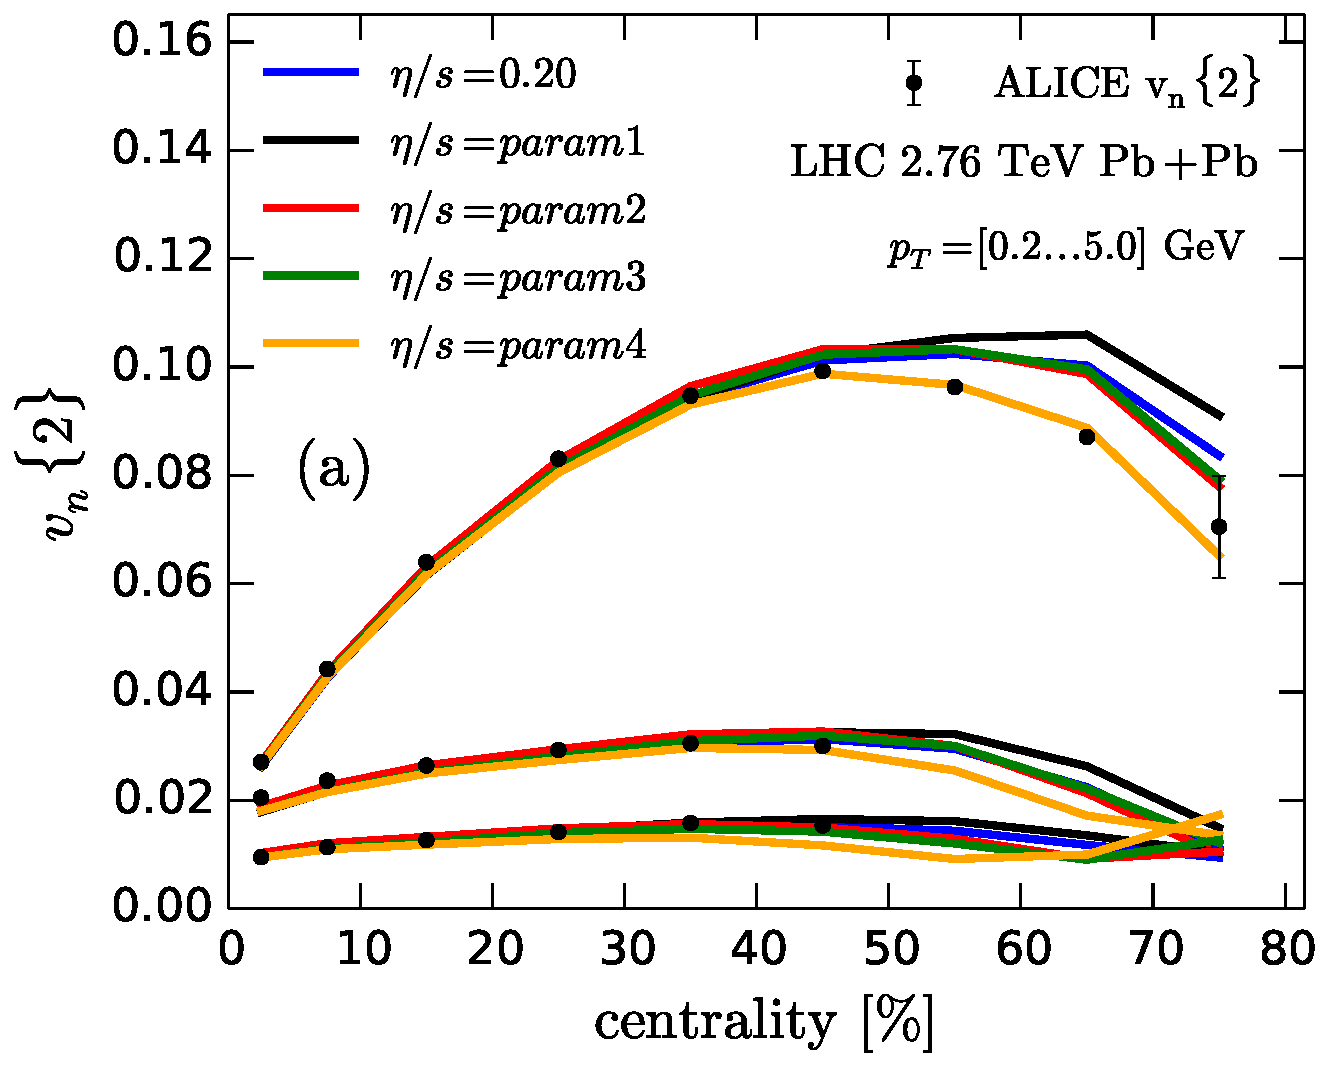
\includegraphics[width=.91\columnwidth]{vn_ekrt} \\
      {\tiny PRC 93, 024907 [1505.02677]}
    \end{column}
    \begin{column}{.075\textwidth}
    \end{column}
  \end{columns}
\end{frame}


\begin{frame}{Not so good in small systems...}
  \centering
  {\tiny PHENIX submitted to PRC [1609.02894]} \\
  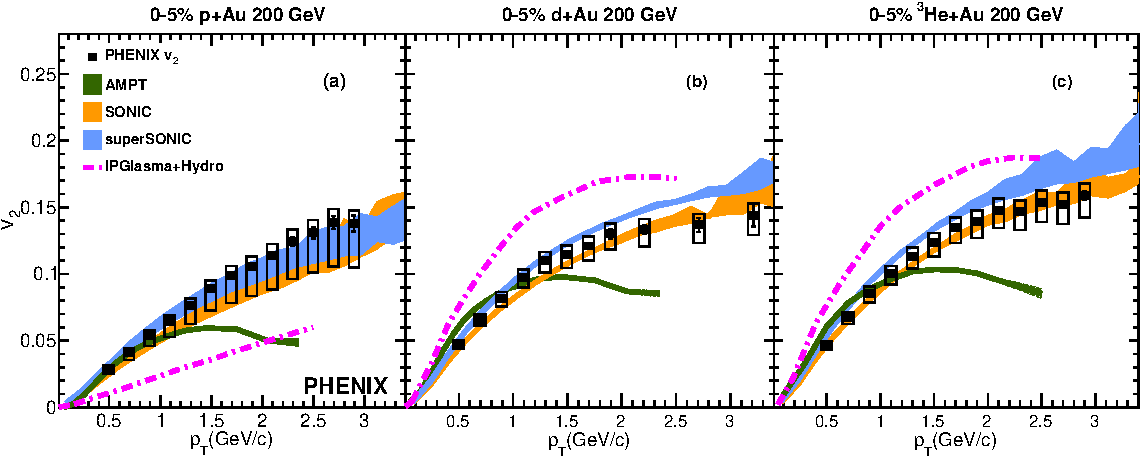
\includegraphics[width=.85\columnwidth]{phenix_models} \\[1ex]
  \small IP-Glasma + hydro could not reproduce experimental\\multiparticle correlations in small systems... what's wrong? \\[1ex]
  \begin{itemize}
    \item Perhaps hydro isn't valid, incorporate initial CGC correlations
    \item SONIC model works quite well, revisit the MC-Glauber model?
    \item Saturation IC + hydro correct picture, small systems require additional nucleon substructure
  \end{itemize}
\end{frame}

\begin{frame}{"Eccentric protons?" \quad {\scriptsize \textcolor{offblack}{Schenke, Venugopalan PRL 113 102301}}}
  \small
  \begin{itemize}
    \item Data highly constrains functional form of initial entropy deposition (talk by J.\ Bernhard).\\[1ex]
    \item Cannot modify the mapping without spoiling bulk A+A observables, but \emph{we can} add
          fine structure to the inputs (thickness functions)\\[2ex]
  \end{itemize}
  \centering
  \only<1>{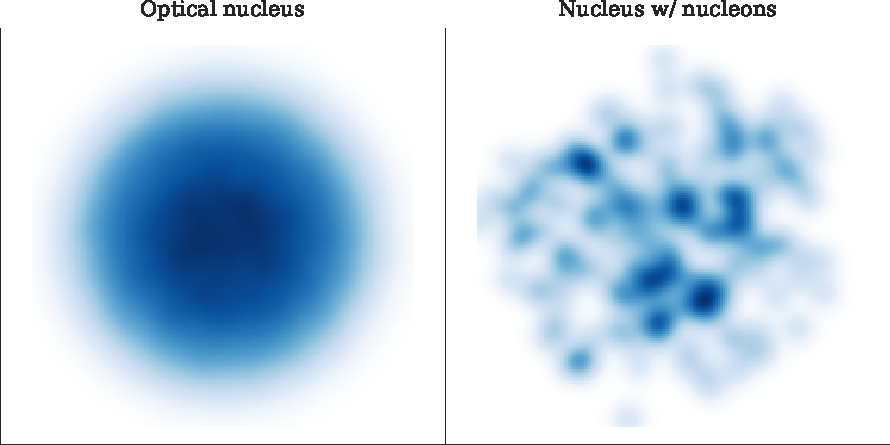
\includegraphics[width=.8\textwidth]{Pb_thick}}
  \only<2>{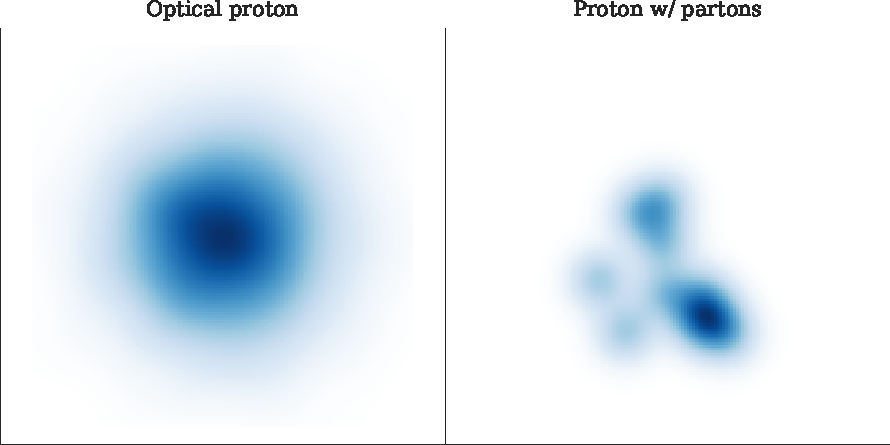
\includegraphics[width=.8\textwidth]{p_thick}} \\[2ex]
  \only<1>{Historical analogue: nucleon position hot spots necessary for $v_3$}
  \only<2>{Possibly similar picture for partons inside the nucleon?}

\end{frame}

\begin{frame}
  \begin{columns}
    \begin{column}{.8\textwidth}
    \centering
    {\Large Objective:}\\[1ex]
    \begin{itemize}
      \item Extend \trento\ initial conditions to include nucleon substructure\\[1ex]
      \item Estimate new substructure parameters using Bayesian methodology 
    \end{itemize}
    \end{column}
  \end{columns}
\end{frame}


\begin{frame}{\protect\trento: parametric initial condition model}
    \only<1>{
    \begin{tikzpicture}[remember picture,overlay]
        \node[anchor=center, xshift=-2 cm, yshift=0.9 cm] at (current page.center) {
            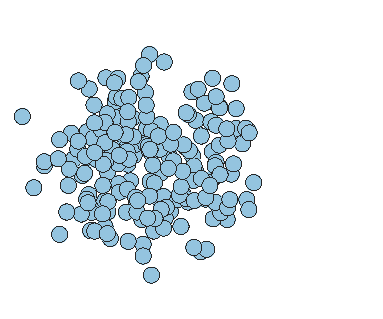
\includegraphics[scale=1]{nucleusB}};
        \node[anchor=center, xshift= 2 cm, yshift=0.9 cm] at (current page.center) {
            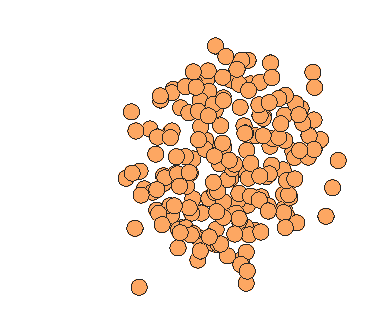
\includegraphics[scale=1]{nucleusA}};
        \node[below = 2.5 cm of current page.center, anchor=center, align=center]{Sample nucleon positions};
    \end{tikzpicture}}
   
    \only<2>{ 
    \begin{tikzpicture}[remember picture,overlay]
        \node[anchor=center, yshift=0.9 cm] at (current page.center) {
            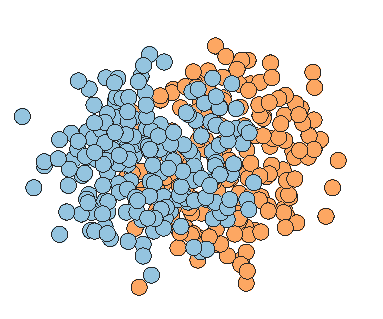
\includegraphics[scale=1]{nucleusAB}};
        \node[below = 2.5 cm of current page.center, anchor=center, align=center]{
          Nuclei collide at random impact parameter $b$ \\[1ex]
          $dP(b) = 2 \pi b\, db$};
    \end{tikzpicture}}
    
    \only<3>{ 
    \begin{tikzpicture}[remember picture,overlay]
        \node[anchor=center, yshift=0.9 cm] at (current page.center) {
            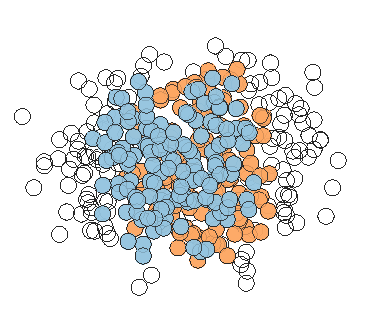
\includegraphics[scale=1]{partAB}};
        \node[below = 2.5 cm of current page.center, anchor=center, align=center] {
          Determine participants by pairwise collision probability \\[1ex]
          $P_\mathrm{coll}(b) = 1 - \exp\big[{-}\sigma_\mathrm{partonic} T_{pp}(b)\big]$
        };
    \end{tikzpicture}}
    
    \only<4>{
    \begin{tikzpicture}[remember picture,overlay]
        \node[anchor=center, xshift=-2 cm, yshift=0.9 cm] at (current page.center) {
            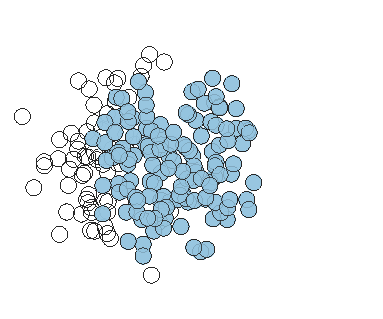
\includegraphics[scale=1]{partB}};
        \node[anchor=center, xshift= 2 cm, yshift=0.9 cm] at (current page.center) {
            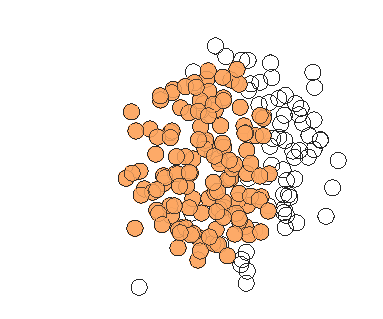
\includegraphics[scale=1]{partA}};
        \node[below = 2.7 cm of current page.center, anchor=center, align=center]{
          Construct participant thickness functions \\[1ex]
          $\tilde{T}_{A,B} = \sum\limits_{i=1}^{N_\mathrm{part}} w_i T_p(\mathbf{x} - \mathbf{x}_i)$ \\[1ex]
          using Gamma random weights $w_i$};
    \end{tikzpicture}}
    
    \only<5>{
    \begin{tikzpicture}[remember picture,overlay]
        \node[anchor=center, xshift=-2 cm, yshift=0.9 cm] at (current page.center) {
            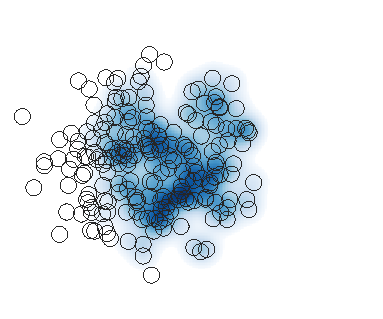
\includegraphics[scale=1]{thickB}};
        \node[anchor=center, xshift= 2 cm, yshift=0.9 cm] at (current page.center) {
            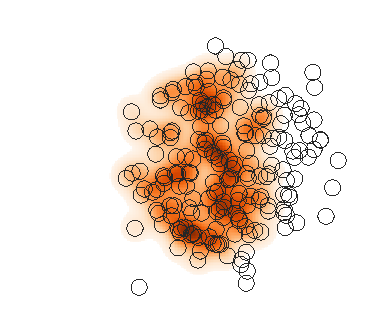
\includegraphics[scale=1]{thickA}};
        \node[below = 2.7 cm of current page.center, anchor=center, align=center]{
          Construct participant thickness functions\\[1ex]
          $\tilde{T}_{A,B} = \sum\limits_{i=1}^{N_\mathrm{part}} w_i T_p(\mathbf{x} - \mathbf{x}_i)$ \\[1ex]
        using Gamma random weights $w_i$};
    \end{tikzpicture}}
    
    \only<6>{
    \begin{tikzpicture}[remember picture,overlay]
        \node[anchor=center, yshift=0.9 cm] at (current page.center) {
            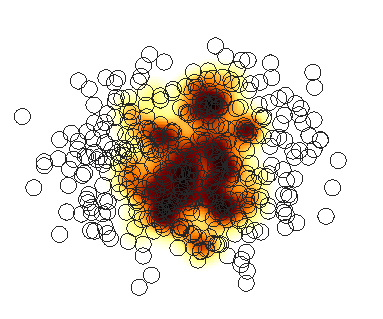
\includegraphics[scale=1]{entropy}};
        \node[below = 2.8 cm of current page.center, align=center, anchor=center]{
          Deposit entropy according to eikonal parametrization: \\[1ex]
            $\dfrac{dS}{dy}\,\Bigg\vert_{\tau=\tau_0} \propto \Bigg(\dfrac{\tilde{T}_A^p + \tilde{T}_B^p}{2}\Bigg)^{1/p}$ \\[1.5ex]
            \emph{generalized mean of participant nuclear density}
        };
    \end{tikzpicture}}
    
\end{frame}


\begin{frame}{Parametrizing local entropy deposition}
    \centering \bigskip
    \begin{tcolorbox}[colback=theme!10, colframe=theme!0]
        \centering \small Generalized mean ansatz: \quad
                   $\displaystyle \frac{dS}{d^2r\, dy} \propto
                    \biggl(\frac{T_A^p + T_B^p}{2}\biggr)^{1/p}$
            \tikz[remember picture] \node[coordinate, above=5 pt] (d1) {};
    \end{tcolorbox}
    \smallskip
    \begin{columns}[T]
        \begin{column}{0.05\textwidth}
        \end{column}
        \begin{column}{0.75\textwidth}
            \centering
            \includegraphics<1>[width=\textwidth]{thickness_band} 
            \includegraphics<2>[width=\textwidth]{thickness_arithmetic} 
            \includegraphics<3>[width=\textwidth]{thickness_geometric} 
            \includegraphics<4>[width=\textwidth]{thickness_harmonic} 
        \end{column}
        \begin{column}{0.15\textwidth}
            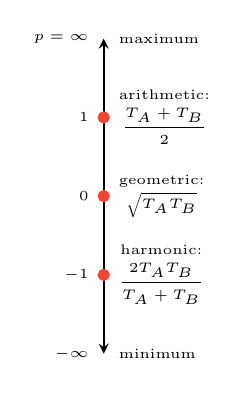
\begin{tikzpicture}
                \tiny
                \tikz[remember picture] \node[coordinate, left=5pt, above=5pt] (d2) {};
                \draw[semithick, <->, >=stealth] (0,0) -- (0,-4);
                \foreach \y in {-1,-2,-3} \draw[semithick] (-2pt, \y cm) -- (2pt, \y cm);
                \draw (0,0) node[left=3pt] {$p=\infty$} node[right=3pt] {maximum};
                \draw (0,-1) node[left=3pt] {$1$} node[right=3pt, align=center] {
                    arithmetic:\\[1ex] $\displaystyle \frac{T_A+T_B}{2}$};
                \draw (0,-2) node[left=3pt] {$0$} node[right=3pt, align=center] {
                    geometric:\\[.4ex] $\displaystyle \sqrt{T_A T_B}$};
                \draw (0,-3) node[left=3pt] {$-1$} node[right=3pt, align=center] {
                    harmonic:\\[1ex] $\displaystyle \frac{2 T_A T_B}{T_A + T_B}$};
                \draw (0,-4) node[left=3pt] {$-\infty$} node[right=3pt] {minimum};
                \draw<2>[pyred, fill=pyred] (0,-1) circle (2 pt);
                \draw<3>[pyred, fill=pyred] (0,-2) circle (2 pt);
                \draw<4>[pyred, fill=pyred] (0,-3) circle (2 pt);
            \end{tikzpicture} 
        \end{column}
        \begin{column}{0.05\textwidth}
        \end{column}
    \end{columns}

    \begin{tikzpicture}[remember picture, overlay]
        \path[->, >=stealth, theme] (d1) edge [out=-45, in=45] (d2);
    \end{tikzpicture}
\end{frame}


\begin{frame}{Sampling partons inside the proton}
  \begin{columns}
    \begin{column}{.4\textwidth}
      \textbf{Variable parameters:}
      \begin{itemize}
        \item Nucleon width
        \item Parton width
        \item Number of partons
      \end{itemize}
      \bigskip
      \textbf{Necessary constraints:}
      \begin{itemize}
        \item Fit inelastic p+p \\
              cross section
        \item Preserve avg proton radial distribution
      \end{itemize}
    \end{column}
    \vline \hspace{1 cm}
    \begin{column}{.5\textwidth}
      \begin{block}{Procedure}
        \scriptsize
        \begin{enumerate}
          \item Sample parton radius $v$ from deconvolved proton radius $w$ \\[1ex]
                $r_\mathrm{sample} = \sqrt{w^2 - v^2}$
          \item Given a nucleon pair, take all possible parton pairs.
                Parton pair collision prob given by:\\[1ex]
                $P_\mathrm{coll} = 1 - \exp(-\sigma_{pp} T_{pp})$
          \item Nucleon pair collides if one or more parton pairs collide.\\[1ex]
                \emph{All partons} in participant nucleon added to nucleon
                thickness function.
              \item Partonic cross section parameter $\sigma_{pp}$ is numerically
                tuned to fit $\sigma^\mathrm{inel}_{nn}$ \\[1ex]
                $\sigma_{nn}^\mathrm{inel} = \int d^2b\, \big[1 - \prod\limits_{i,j} \,P_\mathrm{miss}^{\,ij}\big]$
        \end{enumerate}
      \end{block}
    \end{column}
  \end{columns}
\end{frame}


\begin{frame}{Effect on nuclear thickness functions}
  \begin{columns}
    \begin{column}{.02\textwidth}
      \rotatebox{90}{\small Parton width [fm]}
    \end{column}
    \begin{column}{.49\textwidth}
      \centering Lead nucleus \\ 
      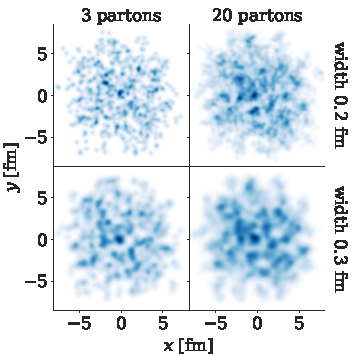
\includegraphics[height=\columnwidth]{Pb_thickness} \\
      \small Parton number
    \end{column}
    \begin{column}{.49\textwidth}
      \centering Proton \\
      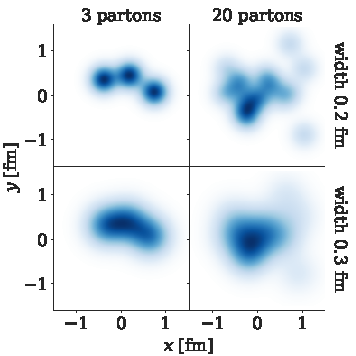
\includegraphics[height=\columnwidth]{p_thickness} \\
      \small Parton number
    \end{column}
  \end{columns}
  \vspace{.75 cm}
  \centering
  \small nucleon width fixed, $w = 0.5$~fm
\end{frame}

\begin{frame}{Exploring the parameter space}
  \centering
  \medskip
  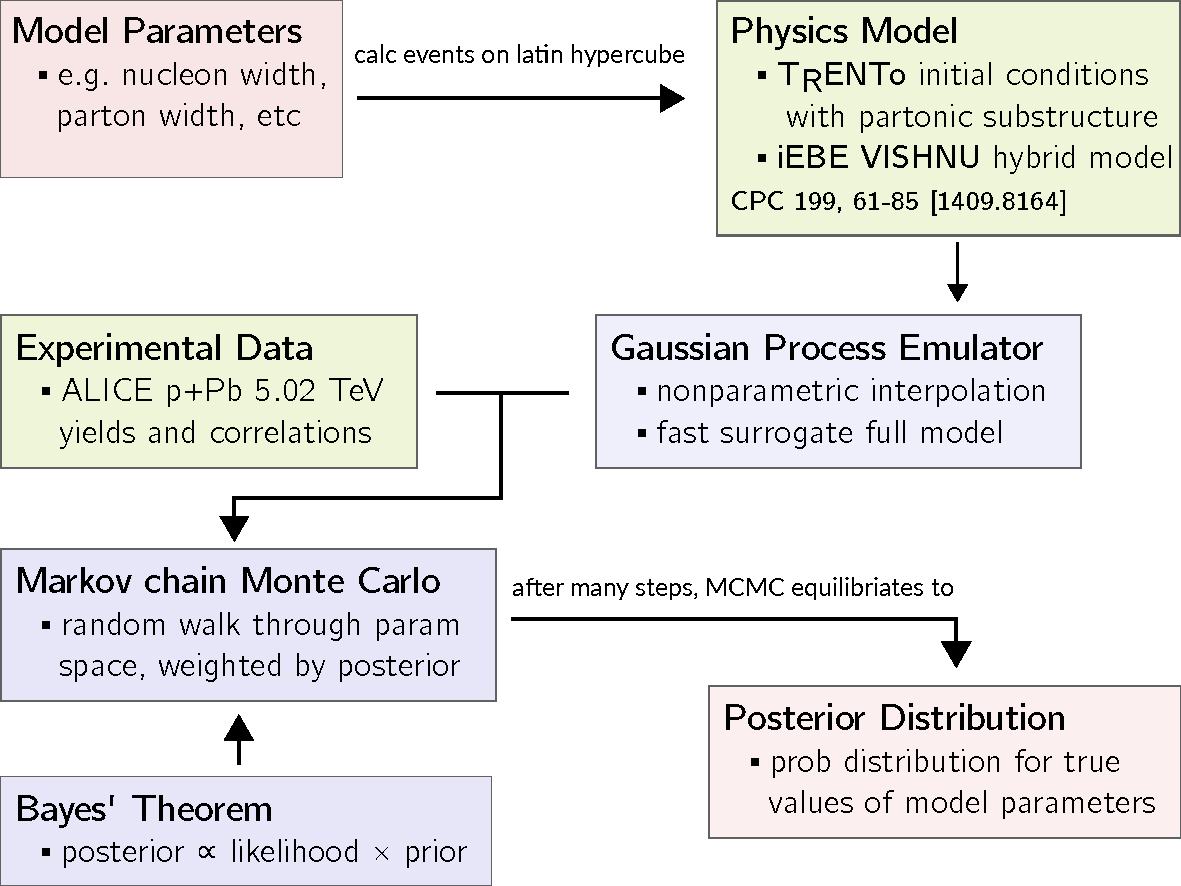
\includegraphics[width=.95\textwidth]{flowchart} \\
\end{frame}


\begin{frame}{Creating the design space}
  \begin{columns}
    \begin{column}{.05\textwidth}
    \end{column}
    \begin{column}{.45\textwidth}
      \smallskip \\
      \textbf{parton number} \\[1ex]
      $n_\mathrm{partons} = 2^k$, \\[1ex]
      $k \in 1$--$4.5$ \\[1ex]
      \textbf{nucleon width} \\[1ex]
      $w \in 0.4$--$1$ fm \\[1ex]
      \textbf{parton width:} \\[1ex]
      $v_\mathrm{min} = \sqrt{\frac{A_\mathrm{min}}{n_\mathrm{parton}}}$ \\[1ex]
      $v_\mathrm{max} = w$ \\[1ex]
      $v = v_\mathrm{min} + x\,(v_\mathrm{max} - v_\mathrm{min})$ \\[1ex]
      $x \in [0, 1]$, \quad $A_\mathrm{min} = 0.1$ fm$^2$
    \end{column}
    \begin{column}{.45\textwidth}
      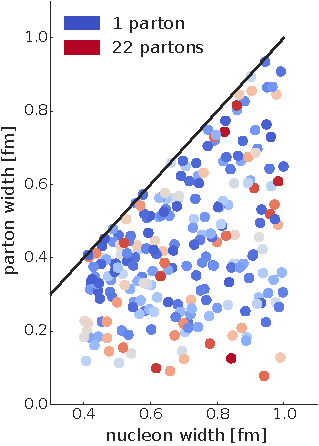
\includegraphics{parameter_design}
    \end{column}
    \begin{column}{.05\textwidth}
    \end{column}
  \end{columns}
\end{frame}

\begin{frame}[t]{Measuring hydrodynamic response}
  \vspace{.5 cm}
  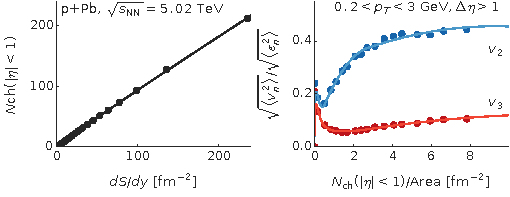
\includegraphics[width=\textwidth]{response}\\
  \begin{enumerate}
    \item Sample IC parameters from design, fix hydro \\
      parameters using Bayesian constraints determined from Pb+Pb collisions (talk by J.\ Bernhard)
    \only<1>{
      \\[1ex]$(\eta/s)_\mathrm{min} = 0.06$,\quad $(\eta/s)_\mathrm{slope} = 2.0$~GeV$^{-1}$,\quad $\tau_\mathrm{fs} = 0.6$ fm/c
      \\[1ex]$(\zeta/s)_\mathrm{max} = 0.015$,\quad $(\zeta/s)_\mathrm{width} = 0.02$~GeV
    }
    \only<2>{
    \item Run $\mathcal{O}(10^4)$ min bias hydro + UrQMD events \\[1ex]
    \item Fit functions for yield, elliptic and triangular flows
    }
  \end{enumerate}
\end{frame}

\begin{frame}[b]{Training data}
  \bigskip
  \begin{itemize}
    \item Lines: model calculations at each design point, \\
      calculated by applying response functions to $dS/dy$ and $\varepsilon_n$ \\[1ex]
    \item Symbols: ALICE 5.02 p+Pb data; central bins combined,\\
      and $v_3$ data interpolated to match $v_2$ centrality bins
  \end{itemize}
  \bigskip
  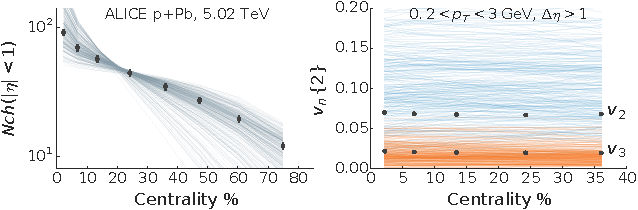
\includegraphics[width=\textwidth]{observables_design} \\[1ex]
  \centering
  {\scriptsize Data: ALICE, PRC 90, 054901 [1406.2474]}
  \vspace{1.2 cm}
\end{frame}

\begin{frame}[t]{Posterior samples}
  \bigskip
  \begin{itemize}
    \item One-hundred samples drawn from the calibrated model \\[1ex]
    \item Spread encapsulates uncertainty in the optimal values of the model parameters
  \end{itemize}
  \bigskip
  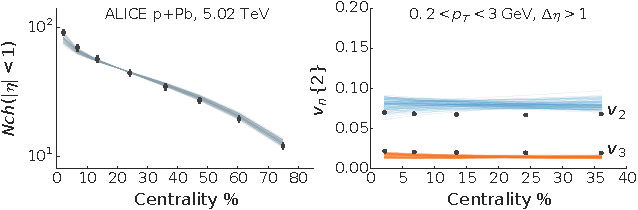
\includegraphics[width=\textwidth]{observables_samples} \\[1ex]
  \centering
  {\scriptsize Data: ALICE, PRC 90, 054901 [1406.2474]}
  \vspace{1.2 cm}
\end{frame}

\begin{frame}[plain]
  \centering
  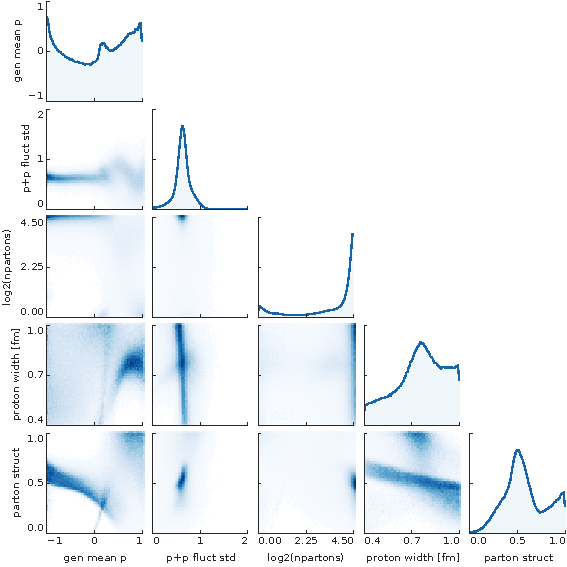
\includegraphics[width=.95\textheight]{posterior}
  \begin{textblock*}{0.6\paperwidth}(5.5 cm, 1 cm)
    {\Large \color{theme}{Posterior distribution}} \\
    \small flat 15\% error on data \\
  \end{textblock*}
  \begin{textblock*}{0.6\paperwidth}(5.5 cm, 2 cm)
    \begin{itemize}
      \item Diagonal: marginalized posterior dist.\\for individual model parameters
    \end{itemize}
  \end{textblock*}
  \begin{textblock*}{0.6\paperwidth}(7.2 cm, 3.2 cm)
    \begin{itemize}
      \item Lower diagonal: joint dist's\\for pairs of parameters
    \end{itemize}
  \end{textblock*}
\end{frame}

\begin{frame}[plain]
  \centering
  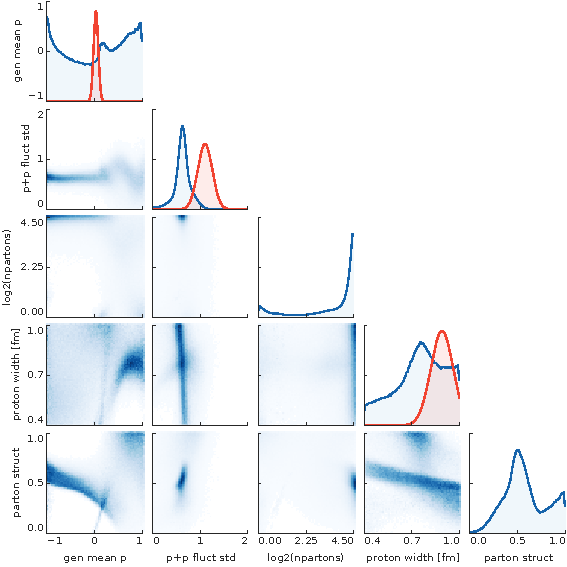
\includegraphics[width=.95\textheight]{posterior_jonah}
  \begin{textblock*}{0.6\paperwidth}(5.5 cm, 1 cm)
    {\Large \color{theme}{Posterior distribution}} \\
    \small flat 15\% error on data \\
  \end{textblock*}
  \begin{textblock*}{0.6\paperwidth}(5.5 cm, 2 cm)
    \begin{itemize}
      \item Diagonal: marginalized posterior dist.\\for individual model parameters
    \end{itemize}
  \end{textblock*}
  \begin{textblock*}{0.6\paperwidth}(7.2 cm, 3.2 cm)
    \begin{itemize}
      \item Lower diagonal: joint dist's\\for pairs of parameters
    \end{itemize}
  \end{textblock*}
  \begin{textblock*}{0.6\paperwidth}(7.9 cm, 4.4 cm)
    \begin{itemize}
      \item Red: prior information\\
        from Pb+Pb analysis \\[.3em]
            \hspace{1.5 cm} \scriptsize PRC 94, 024907
    \end{itemize}
  \end{textblock*}
\end{frame}

\begin{frame}[plain]{Posterior nucleon realizations}
  \smallskip
  \begin{tabular}{ll}
    Nucleon width & $w = 0.88$~fm \\
    Parton number & $m = 22$ \\
    Parton width & $v = 0.45$~fm \\[1ex]
  \end{tabular}
  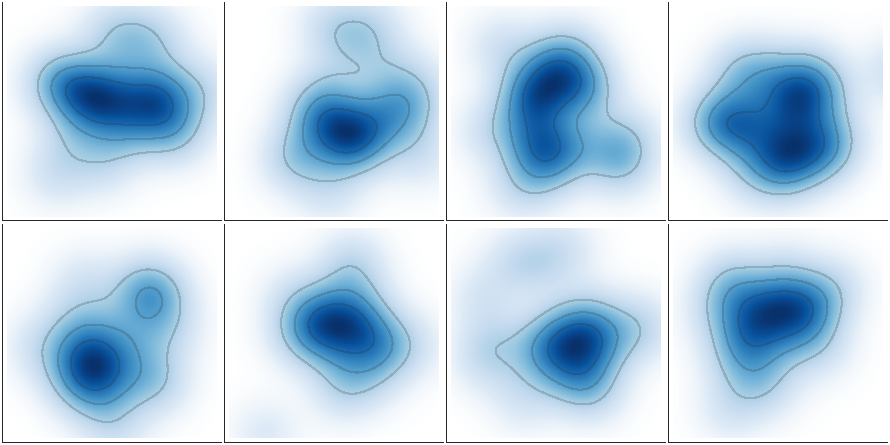
\includegraphics[width=\textwidth]{posterior_protons} \\[1ex]
  \centering
  \small Proton thickness functions $[\mathrm{fm}^{-2}]$
\end{frame}

\begin{frame}{Summary and Outlook}
  \large Presented \\
  \begin{itemize}
    \small
    \item Added variable parton number, width to nuclear thickness func's
    \item Proton--lead collisions appear to prefer many partons (${>}10$)
    \item No clear tension in A+A and p+A parameters using substructure
    \item Current estimates slightly overshoot gap between $v_2$ and $v_3$
  \end{itemize}
  \large To do \\
  \begin{itemize}
    \small
    \item Replace response function with e-by-e hydro+micro
    \item Calibrate to Pb+Pb and p+Pb simultaneously
    \item Increase max partons to $\sim\!100$
    \item Add observables, e.g.\ mean $p_T$, and additional collision systems
  \end{itemize}

\end{frame}

\appendix


\begin{frame}{QGP initial conditions in the Eikonal approximation}
  \begin{columns}
    \begin{column}{.8\textwidth}
      \begin{assertion}
        \small Initial energy (entropy) deposition is \underline{local} \\[1ex]
        Sees only transverse nuclear densities $T_{A,B}$ \\[1ex]
        Hence \quad $\dfrac{d^2S}{dx^2\tau_0 d\eta}\Biggr\vert_{\eta=0} \approx f(T_A, T_B)$
      \end{assertion}
      \vspace{.6 cm}
      The mapping\, $f: T_A, T_B \mapsto s(\mathbf{x}, \eta)$ should be \emph{universal} at a given beam energy!\\
      \medskip
      ...should not change across p+p, p+Pb, Pb+Pb systems at $\sqrt{s_\mathrm{NN}} = \text{const}$.
    \end{column}
  \end{columns}
\end{frame}


\begin{frame}[t]{\trento: comparing to specific models}
  \begin{columns}
    \begin{column}{.4\textwidth}
      \centering
      \vspace{0.3 cm}\\
      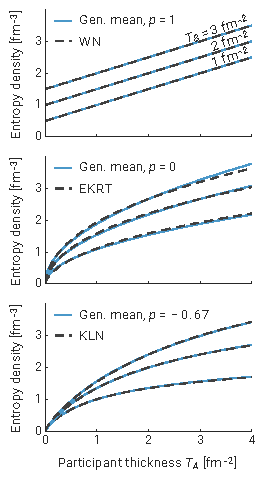
\includegraphics[width=.95\columnwidth]{cgc_compare}
    \end{column}
    \begin{column}{.6\textwidth}
      \vspace{-0.75 cm}
      \begin{itemize}
        \item Wounded nucleon model \\[1ex]
          $\dfrac{dS}{dy d^2r_\perp} \propto T_A + T_B$ \\[1ex]
          \emph{\scriptsize $^*T$ denotes participant thickness} \\[2ex]
        \item EKRT model \quad \textcolor{theme}{\scriptsize PRC 93, 024907} \\[1ex]
          $\dfrac{dE_T}{dy d^2r_\perp} \sim \dfrac{K_\mathrm{sat}}{\pi} p_\mathrm{sat}^3(K_\mathrm{sat}, \beta; T_A, T_B)$ \\[1ex]
          \emph{\scriptsize after brief free streaming phase} \\[2ex]
        \item KLN model \quad \textcolor{theme}{\scriptsize PRC 75, 034905} \\[1ex]
          $\dfrac{dN_g}{dy d^2r_\perp} \sim Q_{s,\mathrm{min}}^2 \Bigg[2 + \log\Bigg(\dfrac{Q_{s,\mathrm{max}}^2}{Q_{s,\mathrm{min}}^2}\Bigg)\Bigg]$\\[1ex]
      \end{itemize}
    \end{column}
  \end{columns}
\end{frame}


\begin{frame}{Establishing priorities in model-to-data comparison}
  \begin{columns}
    \begin{column}{.4\textwidth}
      \centering
      Model-to-data hierarchy \\[1ex]
      \scriptsize \emph{find the IC mapping $f$ which describes,} \\[1ex]
      $\downarrow$ \\[1ex]
      Yields in large, then small systems \\[1ex] 
      $\downarrow$ \\[1ex]
      Correlations in large systems \\[1ex]
      $\downarrow$ \\[1ex]
      Correlations in p+p, p+A? \\[1ex]
      \emph{$^*$hydrodynamic danger zone} \\
      \bigskip
      \begin{block}{\scriptsize Prioritize observables logically}
        \vspace{-.1 cm}
        \begin{itemize}
          \item simple to complex\\
          \item macroscopic to microscopic
        \end{itemize}
      \end{block}
    \end{column}
    \begin{column}{.5\textwidth}
      \centering
      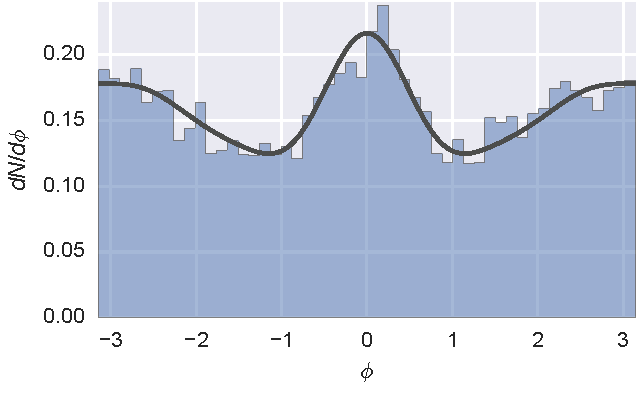
\includegraphics[width=\textwidth]{yields} \\[1ex]
      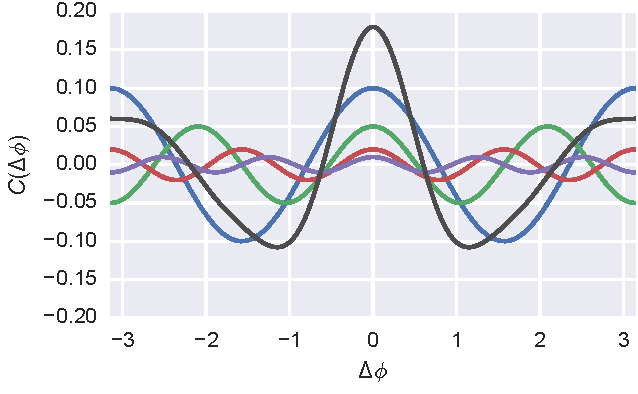
\includegraphics[width=\textwidth]{harmonics}
    \end{column}
  \end{columns}
\end{frame}


\begin{frame}[plain]{Nucleon substructure---a new degree of freedom}
  \vspace{.2 cm}
  \small \centering  PRC 87 064906 [1304.3403v3] \\[1ex]
  \begin{columns}
    \begin{column}{.05\textwidth}
    \end{column}
    \begin{column}{.95\textwidth}
      \begin{flushleft}
        \only<1>{
          \rotatebox{90}{\Large \hspace{.4 cm} Schematic} \hspace{.5 cm}
          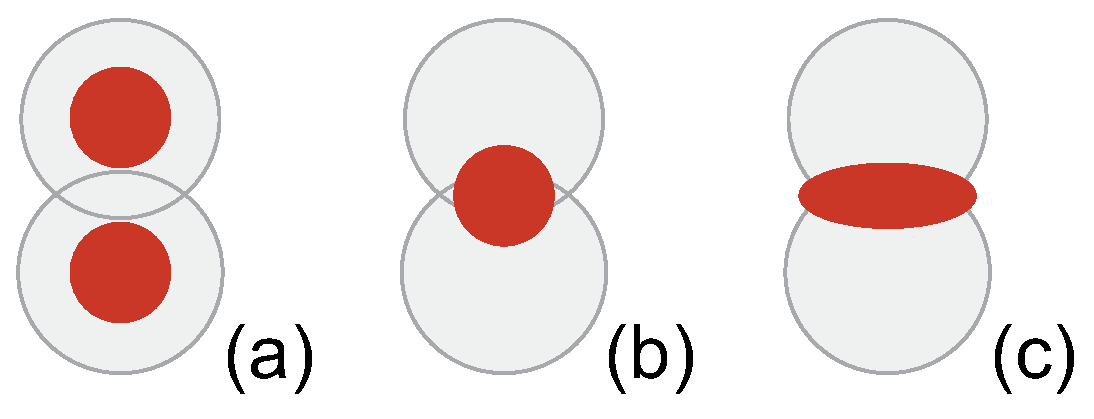
\includegraphics[width=.8\columnwidth]{3models} \\[1ex]
          \rotatebox{90}{\Large \hspace{1 cm} \trento}
          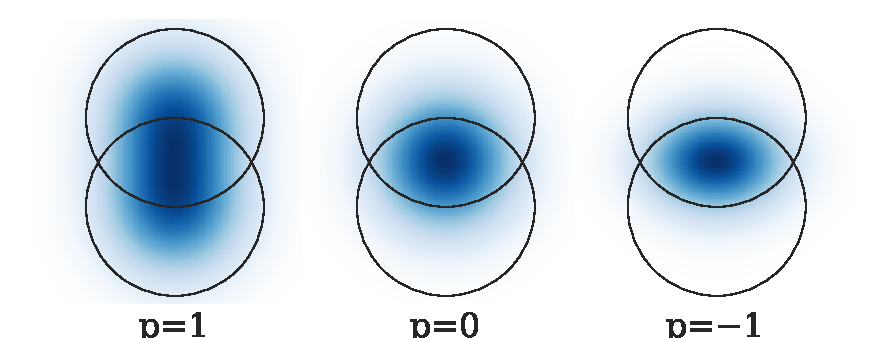
\includegraphics[width=.85\columnwidth]{proton_shapes_gaussian}
        }
        \only<2>{
          \rotatebox{90}{\Large \hspace{.4 cm} Schematic} \hspace{.5 cm}
          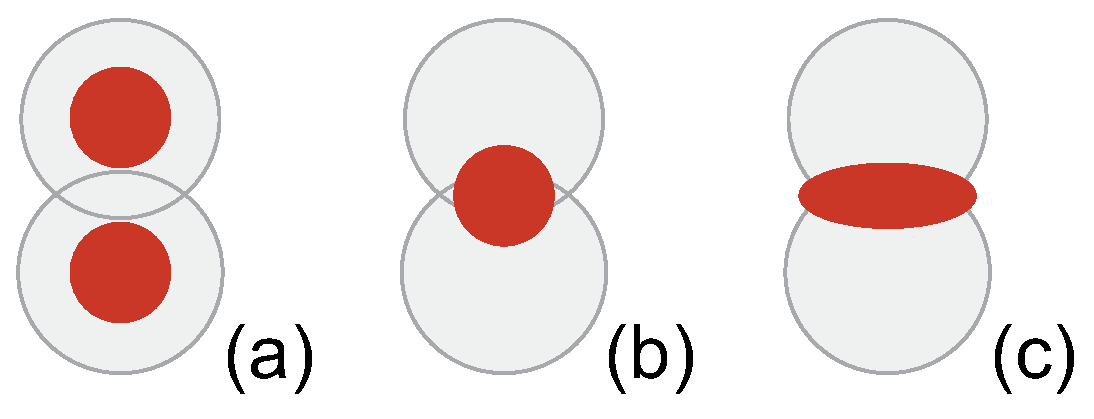
\includegraphics[width=.8\columnwidth]{3models} \\[1ex]
          \rotatebox{90}{\Large \hspace{1 cm} \trento}
          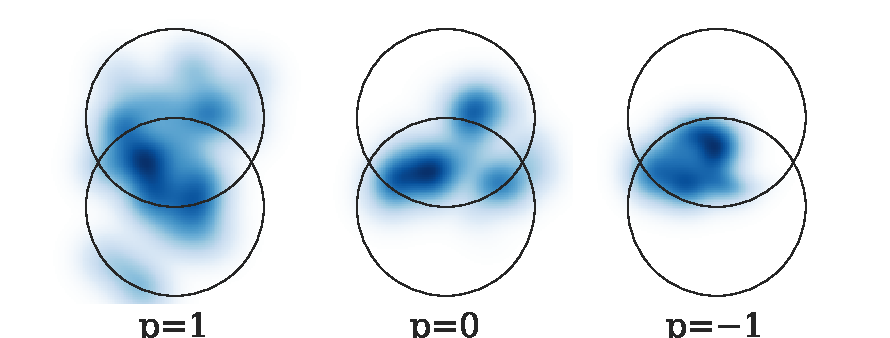
\includegraphics[width=.85\columnwidth]{proton_shapes_substructure}
        }
      \end{flushleft}
    \end{column}
  \end{columns}
\end{frame}


\begin{frame}{Constraining initial conditions in A+A collisions}
  \medskip
  \begin{columns}
    \scriptsize
    \begin{column}{.65\textwidth}
      \centering
      Identified yields, mean $p_T$ and flows \\[1ex]
      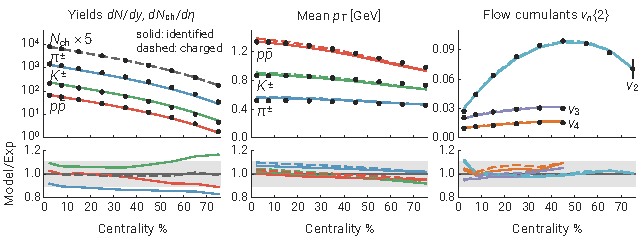
\includegraphics[width=\columnwidth]{mode_observables}
    \end{column}
    \begin{column}{.35\textwidth}
      \centering
      Charged particle yields \\[1ex]
      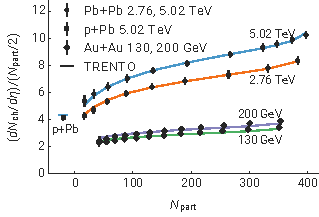
\includegraphics[width=\columnwidth]{nch_per_npart}
    \end{column}
  \end{columns}
  \medskip
  \begin{columns}
    \scriptsize
    \begin{column}{.55\textwidth}
      \centering
      Flow correlations \\[1ex]
      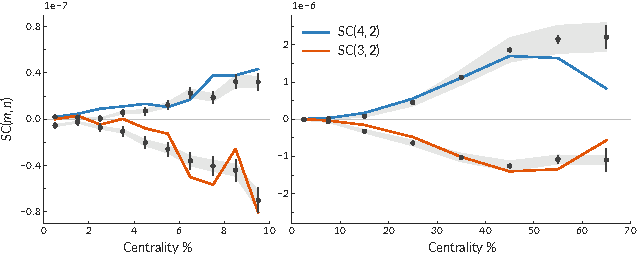
\includegraphics[width=\columnwidth]{flow_corr}
    \end{column}
    \begin{column}{.45\textwidth}
      \centering
      ...all provide strong constraints on IC \\[1ex]
      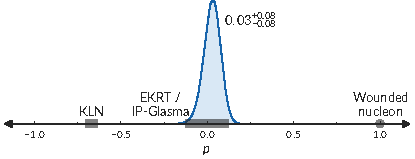
\includegraphics[width=\columnwidth]{posterior_p}
    \end{column}
  \end{columns}
  \vspace{.6 cm}
  \scriptsize
  \centering
  \emph{See talk by J.\ Bernhard for latest results with multiple beam energies,\\
        Tuesday, 11:20 AM, parallel session 2.1}
\end{frame}


\usebackgroundtemplate{%
  \tikz[overlay, remember picture] \node[opacity=1, at=(current page.center), xshift=4 cm, yshift=1.5 cm] {
    
\includegraphics[width=.3\paperwidth]{cover_img}};
}

\begin{frame}{Many models, many approaches}
  First principle calculations, e.g. \\
  \begin{itemize}
    \item IP-Glasma \quad {\scriptsize PRL 108, 252301 [1202.6646]}
    \item EKRT \quad {\scriptsize Nucl.\ Phys.\ B 570, 379--389 [9909456]}
    \item KLN \quad {\scriptsize PRC 74, 044905 [0605012]}
    \item EPOS \quad {\scriptsize PRC 92, 034906 [1306.0121]}
  \end{itemize}
  Parametric models \\
  \begin{itemize}
    \item MC Glauber \quad {\scriptsize Ann.\ Rev.\ Nucl.\ Part.\ Sci.\ 57, 205--243 [0701025]}
    \item \trento\ \quad {\scriptsize PRC 92, 011901 [1412.4708]}
  \end{itemize}
  \bigskip
  All models effectively implement $f: T_A, T_B \mapsto e(\mathbf{x}, \eta)$\\[1ex] 
  Can compare different model calculations though mapping $f$
\end{frame}

\usebackgroundtemplate{}
\end{document}
